% Options for packages loaded elsewhere
\PassOptionsToPackage{unicode}{hyperref}
\PassOptionsToPackage{hyphens}{url}
\PassOptionsToPackage{dvipsnames,svgnames,x11names}{xcolor}
%
\documentclass[
  letterpaper,
  DIV=11,
  numbers=noendperiod]{scrartcl}

\usepackage{amsmath,amssymb}
\usepackage{iftex}
\ifPDFTeX
  \usepackage[T1]{fontenc}
  \usepackage[utf8]{inputenc}
  \usepackage{textcomp} % provide euro and other symbols
\else % if luatex or xetex
  \usepackage{unicode-math}
  \defaultfontfeatures{Scale=MatchLowercase}
  \defaultfontfeatures[\rmfamily]{Ligatures=TeX,Scale=1}
\fi
\usepackage{lmodern}
\ifPDFTeX\else  
    % xetex/luatex font selection
\fi
% Use upquote if available, for straight quotes in verbatim environments
\IfFileExists{upquote.sty}{\usepackage{upquote}}{}
\IfFileExists{microtype.sty}{% use microtype if available
  \usepackage[]{microtype}
  \UseMicrotypeSet[protrusion]{basicmath} % disable protrusion for tt fonts
}{}
\makeatletter
\@ifundefined{KOMAClassName}{% if non-KOMA class
  \IfFileExists{parskip.sty}{%
    \usepackage{parskip}
  }{% else
    \setlength{\parindent}{0pt}
    \setlength{\parskip}{6pt plus 2pt minus 1pt}}
}{% if KOMA class
  \KOMAoptions{parskip=half}}
\makeatother
\usepackage{xcolor}
\setlength{\emergencystretch}{3em} % prevent overfull lines
\setcounter{secnumdepth}{5}
% Make \paragraph and \subparagraph free-standing
\makeatletter
\ifx\paragraph\undefined\else
  \let\oldparagraph\paragraph
  \renewcommand{\paragraph}{
    \@ifstar
      \xxxParagraphStar
      \xxxParagraphNoStar
  }
  \newcommand{\xxxParagraphStar}[1]{\oldparagraph*{#1}\mbox{}}
  \newcommand{\xxxParagraphNoStar}[1]{\oldparagraph{#1}\mbox{}}
\fi
\ifx\subparagraph\undefined\else
  \let\oldsubparagraph\subparagraph
  \renewcommand{\subparagraph}{
    \@ifstar
      \xxxSubParagraphStar
      \xxxSubParagraphNoStar
  }
  \newcommand{\xxxSubParagraphStar}[1]{\oldsubparagraph*{#1}\mbox{}}
  \newcommand{\xxxSubParagraphNoStar}[1]{\oldsubparagraph{#1}\mbox{}}
\fi
\makeatother

\usepackage{color}
\usepackage{fancyvrb}
\newcommand{\VerbBar}{|}
\newcommand{\VERB}{\Verb[commandchars=\\\{\}]}
\DefineVerbatimEnvironment{Highlighting}{Verbatim}{commandchars=\\\{\}}
% Add ',fontsize=\small' for more characters per line
\usepackage{framed}
\definecolor{shadecolor}{RGB}{241,243,245}
\newenvironment{Shaded}{\begin{snugshade}}{\end{snugshade}}
\newcommand{\AlertTok}[1]{\textcolor[rgb]{0.68,0.00,0.00}{#1}}
\newcommand{\AnnotationTok}[1]{\textcolor[rgb]{0.37,0.37,0.37}{#1}}
\newcommand{\AttributeTok}[1]{\textcolor[rgb]{0.40,0.45,0.13}{#1}}
\newcommand{\BaseNTok}[1]{\textcolor[rgb]{0.68,0.00,0.00}{#1}}
\newcommand{\BuiltInTok}[1]{\textcolor[rgb]{0.00,0.23,0.31}{#1}}
\newcommand{\CharTok}[1]{\textcolor[rgb]{0.13,0.47,0.30}{#1}}
\newcommand{\CommentTok}[1]{\textcolor[rgb]{0.37,0.37,0.37}{#1}}
\newcommand{\CommentVarTok}[1]{\textcolor[rgb]{0.37,0.37,0.37}{\textit{#1}}}
\newcommand{\ConstantTok}[1]{\textcolor[rgb]{0.56,0.35,0.01}{#1}}
\newcommand{\ControlFlowTok}[1]{\textcolor[rgb]{0.00,0.23,0.31}{\textbf{#1}}}
\newcommand{\DataTypeTok}[1]{\textcolor[rgb]{0.68,0.00,0.00}{#1}}
\newcommand{\DecValTok}[1]{\textcolor[rgb]{0.68,0.00,0.00}{#1}}
\newcommand{\DocumentationTok}[1]{\textcolor[rgb]{0.37,0.37,0.37}{\textit{#1}}}
\newcommand{\ErrorTok}[1]{\textcolor[rgb]{0.68,0.00,0.00}{#1}}
\newcommand{\ExtensionTok}[1]{\textcolor[rgb]{0.00,0.23,0.31}{#1}}
\newcommand{\FloatTok}[1]{\textcolor[rgb]{0.68,0.00,0.00}{#1}}
\newcommand{\FunctionTok}[1]{\textcolor[rgb]{0.28,0.35,0.67}{#1}}
\newcommand{\ImportTok}[1]{\textcolor[rgb]{0.00,0.46,0.62}{#1}}
\newcommand{\InformationTok}[1]{\textcolor[rgb]{0.37,0.37,0.37}{#1}}
\newcommand{\KeywordTok}[1]{\textcolor[rgb]{0.00,0.23,0.31}{\textbf{#1}}}
\newcommand{\NormalTok}[1]{\textcolor[rgb]{0.00,0.23,0.31}{#1}}
\newcommand{\OperatorTok}[1]{\textcolor[rgb]{0.37,0.37,0.37}{#1}}
\newcommand{\OtherTok}[1]{\textcolor[rgb]{0.00,0.23,0.31}{#1}}
\newcommand{\PreprocessorTok}[1]{\textcolor[rgb]{0.68,0.00,0.00}{#1}}
\newcommand{\RegionMarkerTok}[1]{\textcolor[rgb]{0.00,0.23,0.31}{#1}}
\newcommand{\SpecialCharTok}[1]{\textcolor[rgb]{0.37,0.37,0.37}{#1}}
\newcommand{\SpecialStringTok}[1]{\textcolor[rgb]{0.13,0.47,0.30}{#1}}
\newcommand{\StringTok}[1]{\textcolor[rgb]{0.13,0.47,0.30}{#1}}
\newcommand{\VariableTok}[1]{\textcolor[rgb]{0.07,0.07,0.07}{#1}}
\newcommand{\VerbatimStringTok}[1]{\textcolor[rgb]{0.13,0.47,0.30}{#1}}
\newcommand{\WarningTok}[1]{\textcolor[rgb]{0.37,0.37,0.37}{\textit{#1}}}

\providecommand{\tightlist}{%
  \setlength{\itemsep}{0pt}\setlength{\parskip}{0pt}}\usepackage{longtable,booktabs,array}
\usepackage{calc} % for calculating minipage widths
% Correct order of tables after \paragraph or \subparagraph
\usepackage{etoolbox}
\makeatletter
\patchcmd\longtable{\par}{\if@noskipsec\mbox{}\fi\par}{}{}
\makeatother
% Allow footnotes in longtable head/foot
\IfFileExists{footnotehyper.sty}{\usepackage{footnotehyper}}{\usepackage{footnote}}
\makesavenoteenv{longtable}
\usepackage{graphicx}
\makeatletter
\newsavebox\pandoc@box
\newcommand*\pandocbounded[1]{% scales image to fit in text height/width
  \sbox\pandoc@box{#1}%
  \Gscale@div\@tempa{\textheight}{\dimexpr\ht\pandoc@box+\dp\pandoc@box\relax}%
  \Gscale@div\@tempb{\linewidth}{\wd\pandoc@box}%
  \ifdim\@tempb\p@<\@tempa\p@\let\@tempa\@tempb\fi% select the smaller of both
  \ifdim\@tempa\p@<\p@\scalebox{\@tempa}{\usebox\pandoc@box}%
  \else\usebox{\pandoc@box}%
  \fi%
}
% Set default figure placement to htbp
\def\fps@figure{htbp}
\makeatother

\KOMAoption{captions}{tableheading}
\makeatletter
\@ifpackageloaded{caption}{}{\usepackage{caption}}
\AtBeginDocument{%
\ifdefined\contentsname
  \renewcommand*\contentsname{Table of contents}
\else
  \newcommand\contentsname{Table of contents}
\fi
\ifdefined\listfigurename
  \renewcommand*\listfigurename{List of Figures}
\else
  \newcommand\listfigurename{List of Figures}
\fi
\ifdefined\listtablename
  \renewcommand*\listtablename{List of Tables}
\else
  \newcommand\listtablename{List of Tables}
\fi
\ifdefined\figurename
  \renewcommand*\figurename{Figure}
\else
  \newcommand\figurename{Figure}
\fi
\ifdefined\tablename
  \renewcommand*\tablename{Table}
\else
  \newcommand\tablename{Table}
\fi
}
\@ifpackageloaded{float}{}{\usepackage{float}}
\floatstyle{ruled}
\@ifundefined{c@chapter}{\newfloat{codelisting}{h}{lop}}{\newfloat{codelisting}{h}{lop}[chapter]}
\floatname{codelisting}{Listing}
\newcommand*\listoflistings{\listof{codelisting}{List of Listings}}
\makeatother
\makeatletter
\makeatother
\makeatletter
\@ifpackageloaded{caption}{}{\usepackage{caption}}
\@ifpackageloaded{subcaption}{}{\usepackage{subcaption}}
\makeatother

\usepackage{bookmark}

\IfFileExists{xurl.sty}{\usepackage{xurl}}{} % add URL line breaks if available
\urlstyle{same} % disable monospaced font for URLs
\hypersetup{
  pdftitle={Cryptography},
  colorlinks=true,
  linkcolor={blue},
  filecolor={Maroon},
  citecolor={Blue},
  urlcolor={Blue},
  pdfcreator={LaTeX via pandoc}}


\title{Cryptography}
\author{}
\date{}

\begin{document}
\maketitle

\renewcommand*\contentsname{Table of contents}
{
\hypersetup{linkcolor=}
\setcounter{tocdepth}{3}
\tableofcontents
}

Cryptography has always been about message confidentiality i.e.~making
sure that a message can only be understood by the sender and/or its
intended recipient. It typically involves converting a message into an
incomprehensible format and then that process being reversed by the
recipient. A good cryptography system should leave a potential
eavesdropper with a sense of helplessness i.e.~they should feel like
they don't have the time or energy to figure out what the message is. Of
course the standard for ``time or energy'' has changed drastically with
computers and what seemed like a lot of time or energy doesn't seem like
a lot if you have a computer and know how to write a few scripts.
However, computers also allow us to create even more complicated
encryption systems. Another thing to consider is that even with
computers, there are categories of problems or algorithms that are
difficult for a computer to solve. Recall how complex it was to solve a
towers of hanoi problem (from CSC 220 and CSC/CYEN 131) even when the
algorithm was very simple to write/understand. A good cryptography
system might be easy to understand (i.e.~how it works), but should still
leave us (and our computers) feeling like there isn't enough time/RAM to
figure out the original message.\\
\strut \\
Definitions:

cryptology: enciphering and deciphering

cryptography: making a cipher system

cryptanalysis: breaking a cipher system

encryption: scrambling a message

decryption: unscrambling a message

plain text: original ``readable'' message

cipher text: encrypted ``unreadable'' message

cipher: algorithm for performing encryption or decryption

\paragraph{\texorpdfstring{\textbf{History:}}{History:}}\label{history}

Classic cryptography used pen, paper and perhaps simple mechanical aids.
As we discuss them, try and see if you can figure out how we would break
the cipher and how complicated it might be given current technology
i.e.~current definitions of ``time and energy''. The highlighted
encrypted messages are for you to try and decrypt.\\
\strut \\
- Hieroglyph: 3200BC to about 400AD. Utilized images or symbols to
represent messages that could only be interpreted by those who knew what
the symbols meant. Of course this is no different from writing in a
language. The more people know that language, the less effective it is
at keeping messages secret.\\
\strut \\
- Atbash cipher: 500BC to 1300AD. Its a type of substitution cipher
where the order of the alphabet is reversed i.e.~A becomes Z, B becomes
Y, etc. Examples of it can actually be found in the bible \footnote{(https://www.theology.ox.ac.uk/article/crack-the-code)}.\\
\strut \\

{rhm'g xibkgltizksb ufm?}

\begin{Shaded}
\begin{Highlighting}[]
\NormalTok{$ echo \{z..a\} | tr {-}d \textquotesingle{} \textquotesingle{} \# to create the character set z through a.}
\NormalTok{$ echo "abcde" | tr a{-}z "zyxwvutsrqponmlkjihgfedcba"}
\end{Highlighting}
\end{Shaded}

\begin{itemize}
\tightlist
\item
  Scytale cipher: around 7th century BC. Messages were written on strip
  of parchment wrapped round a rod. When strip was unwrapped, the
  message was unreadable unless it was re-wrapped around a rod of
  similar dimensions.

  {Sdeeeiootyrdnnmhdbwgzeareatostaithoattncimihhbhs}
\item
  Caesar cipher: Also a substitution cipher. Named after the first
  famous person to use this technique. It typically involves replacing a
  character with another character in the same character set but
  identified by shifting the alphabet over by a specific number of
  positions. Caesar used to replace A with D, B with E, C with F,
  \ldots, X with an A, Y with a B, and Z with a C. Because the alphabet
  was rotated by 3 positions, this specific version can be called a
  rot-3 cipher. One of the most common Caesar ciphers is the rot-13
  because the alphabet is reflected i.e.~it is it's own inverse.

  {diwtgh hpxs: durdjght xi xh}
\end{itemize}

\begin{Shaded}
\begin{Highlighting}[]
\NormalTok{$ echo "abcde" | tr a{-}z d{-}za{-}c \#rot{-}3}
\NormalTok{$ echo "abcde" | tr a{-}z n{-}za{-}m \#rot{-}13}
\end{Highlighting}
\end{Shaded}

\begin{itemize}
\tightlist
\item
  Sliding shift cipher: Issue with Caesar is that it is easy to break
  these days. You only need to look at 25 different possibilities to
  decipher it visually. A sliding shift cipher attempts to make this
  more difficult by employing a different shift for each position in the
  plain text string. For example, the first letter is encoded using
  rot-1, second letter using rot-2, third letter using rot-3, etc. One
  doesn't have to start at 1, but the increase size is typically 1.
  However, If I know that the cipher is the sliding shift cipher,
  breaking it is not that hard.\\
  \strut \\
\item
  Vigenere cipher: 1553-1863. Each letter of the plain text was encoded
  by rotating the alphabet based on a key or passphrase. For example, if
  the key was ``key'', then the first letter would be gotten from a
  rot-10 alphabet i.e.~where a became k, b became l, c became m, etc.
  The second letter would be gotten from a rot-4 alphabet i.e.~where a
  became e, b became f, c became g, etc. The key would be repeated as
  many times as necessary to encode the entire plain text. A cipher disk
  or vigenere table (such as the one shown below) can be used for manual
  encryption/decryption. For example, the plain text ``how does this
  work'' can be encrypted using the key ``vigenere''.\\
\end{itemize}

Plain text

H

O

{W}

{D }

{O }

{E }

{S }

{T }

{H}

{I }

{S }

{W }

{O }

{R }

{K}

key

V

I

G

E

N

E

R

E

V

I

G

E

N

E

R

Cipher text

C

W

C

H

B

I

J

X

C

Q

Y

A

B

V

B

\pandocbounded{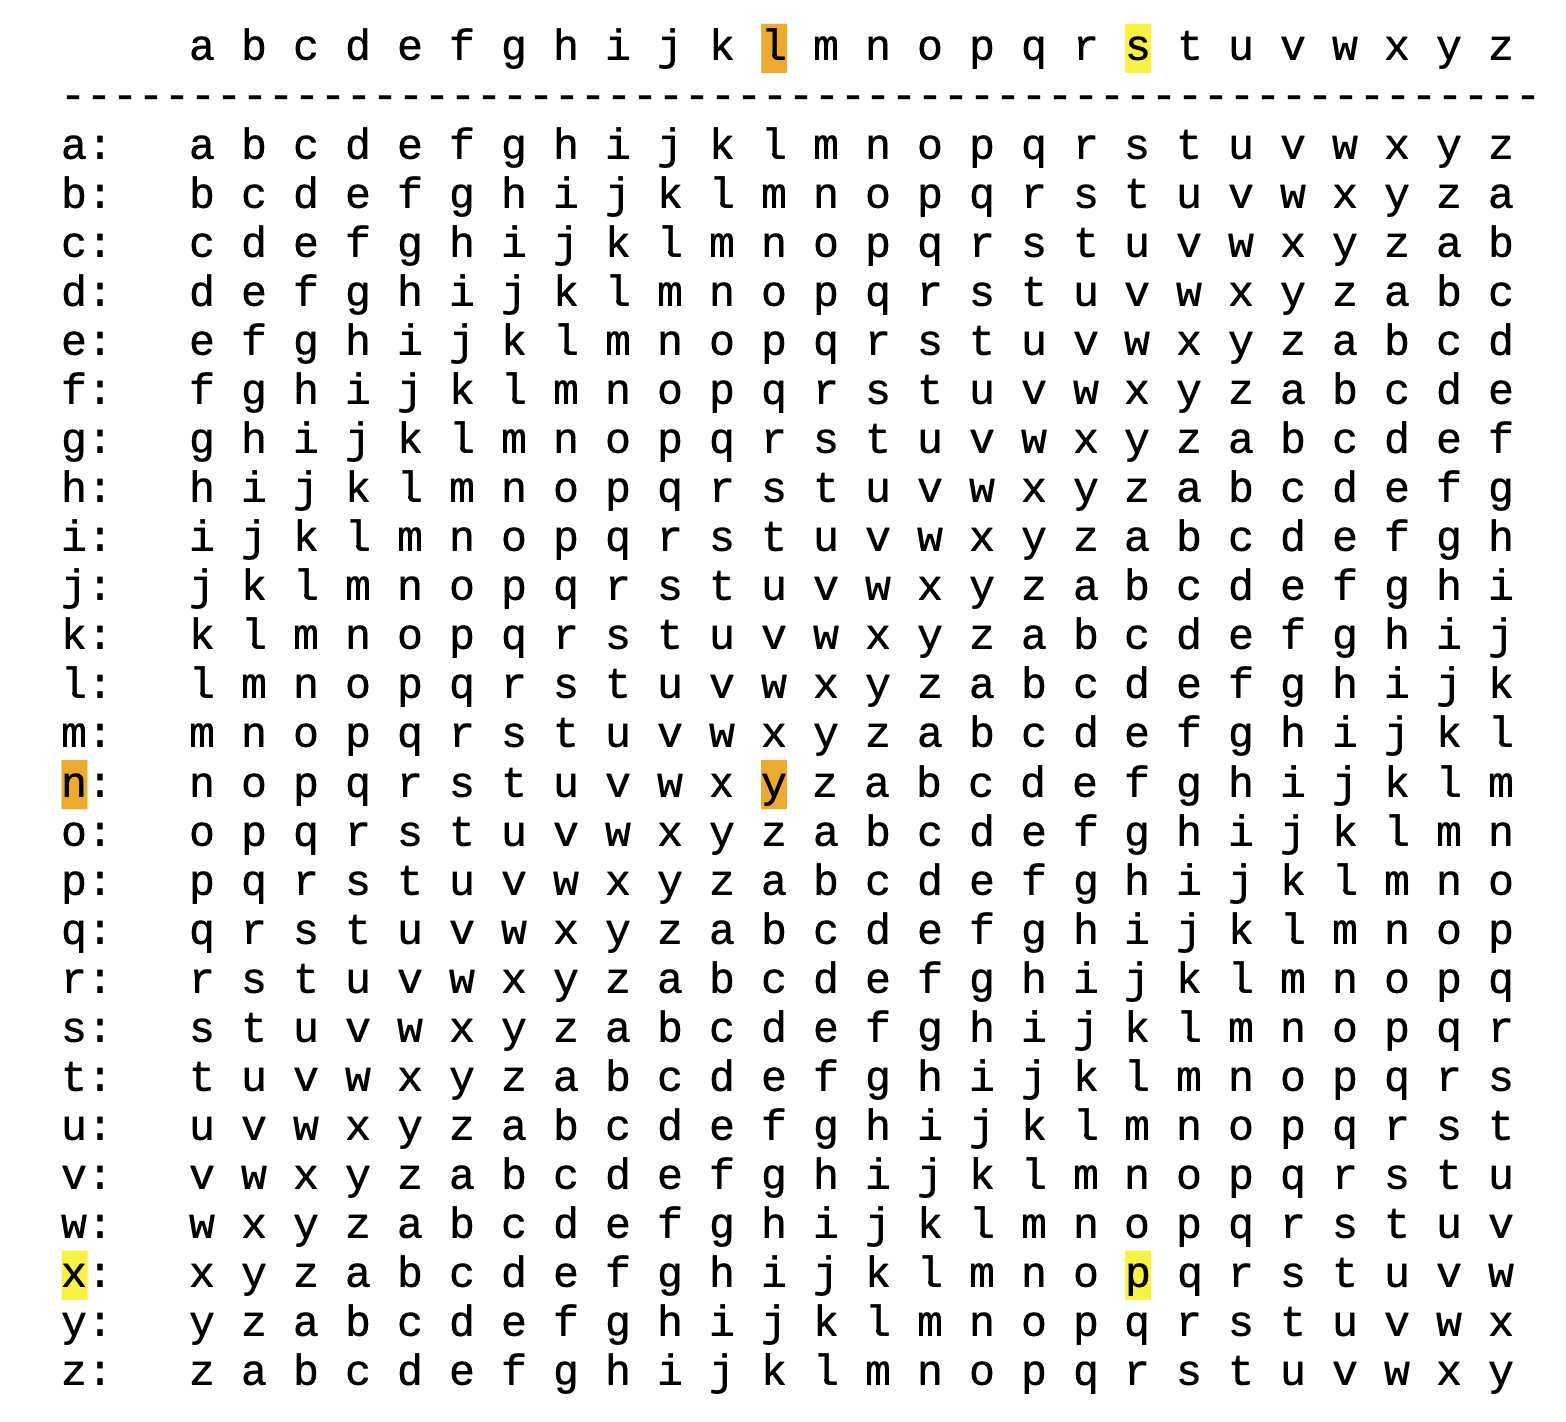
\includegraphics[keepaspectratio]{Plain-key.png}}

In the table above, the column headers is the plain text, and the row
headers is the key, and where the corresponding column and row intersect
is the cipher text. To {encrypt} a plain text character l and key
character n, identify where the column l and row n intersect which is
n.~\\
\strut \\
To {decrypt}, identify the cipher character on the appropriate key row,
and then match it to the corresponding column header. For example, the
cipher character p with the key character x becomes the plain text
character s.\\
\strut \\
Why use manual when we have computers?\\
\strut \\
To take advantage of the computational power now available to us,
however, it is significantly easier/faster if we use math.

A

B

C

D

E

F

G

H

I

J

K

L

M

N

O

P

Q

R

S

T

U

V

W

X

Y

Z

0

1

2

3

4

5

6

7

8

9

10

11

12

13

14

15

16

17

18

19

20

21

22

23

24

25

If we map each character of the plain text and cipher text to a number
(e.g.~the number shown in the table above), then the rotation (or look
up in the vigenere square) is essentially the same as adding those two
numbers and looking up the corresponding letter.\\
\strut \\
For example we see that plain text character l has a value of 11 and key
character n has a value of 13. The sum of those two numbers is 24 which
maps to y. This is an identical result to what we saw with the vigenere
square. If the sum of the two numbers is more than 25, then we wrap
around and continue from the beginning i.e.~\% 26.\\
\strut \\
Decrypting is just a matter of doing the reverse i.e.~subtract the
numerical value of the key character from the numerical value of the
cipher text character to get the numerical value of the plain text
character. Make sure to wrap around if this difference is negative.\\
\strut \\
More formally, if P is the plain text, K the key, C the cipher text, and
the subscript i the character in the ith position of any of those three,
then.

\(C_i=(p_i+K_i)\%26\)\\
\strut \\
To decrypt.\\
\strut \\
\(p_i=(26+C_i-K_i)\%26\)\\
\strut \\
The 26 is added just to make the math of the wrap around consistent
across different programming languages. Some languages give different
results for the modulo of a negative number\\
\strut \\
As an example, if our text is ``cyberstorm is going to be bussin'' and
our key is ``seacreatures''\\

\begin{math}
    \begin{aligned}
    P_0 = c, K_0 = s → C_0 = (2+18)%26 = 20 = u 
    \end{aligned}

    \begin{aligned}
    P_1 = y, K_1 = e → C_1 = (24+4)%26 = 2 = c 
    \end{aligned}

    \begin{aligned}
    P_2 = b, K_2 = a → C_2 = (1+0)%26 = 1 = b 
    \end{aligned}

    \begin{aligned}
    P_3 = e, K_3 = c → C_3 = (4+2)%26 = 6 = g 
    \end{aligned}

    \begin{aligned}
    P_4 = r, K_4 = r → C_4 = (17+17)%26 = 8 = i \nonumber \\
    \end{aligned}

    \begin{aligned}
    P_5 = s, K_5 = e → C_5 = (18+4)%26 = 22 = w \nonumber \\
    \end{aligned}

    \begin{aligned}
    P_6 = t, K_6 = a → C_6 = (19+0)%26 = 19 = t \nonumber \\
    \end{aligned}

    \begin{aligned}
    ...
    \end{aligned}
\end{math}\\
CipherText = \textbf{ucbgiwthld mk ysipx xo uy sykkmn}\\
\strut \\
If you wanted to decrypt ``qis afyr ilfjwkwot lwew vlwkar. Hg'j ixmlr.
Rg uep.'' using the same key.

\begin{math}
    \begin{aligned}
    C_0 = q, K_0 = s → P_0 = (26+16-18)%26 = 24 = y
    \end{aligned}

    \begin{aligned}
    C_1 = i, K_1 = e → P_1 = (26+8-4)%26 = 4 = e
    \end{aligned}

    \begin{aligned}
    C_2 = s, K_2 = a → P_2 = (26+18-0)%26 = 18 = s
    \end{aligned}

    \begin{aligned}
    C_3 = a, K_3 = c → P_3 = (26+0-2)%26 = 24 = y
    \end{aligned}

    \begin{aligned}
    C_4 = f, K_4 = r → P_4 = (26+5-17)%26 = 14 = o
    \end{aligned}

    \begin{aligned}
    C_5 = y, K_5 = e → P_5 = (26+24-4)%26 = 20 = u
    \end{aligned}

    \begin{aligned}
    C_6 = r, K_6 = a → P_6 = (26+17-0)%26 = 17 = r
    \end{aligned}

    \begin{aligned}
    … 
    \end{aligned}
\end{math}

Plain text = \textbf{yes your \ldots{}}\\
\strut \\
Since many programming languages actually store characters as integers,
getting the numerical value of the character from the table above is
often as simple as subtracting the integer value of `A' or `a'.\\
\strut \\
In c++ for example, `P' - `A' = 80 -- 65 = 15.\\
\strut \\
Historically speaking, cryptography was almost always concerned with
hiding written language text. Computers have changed the game in three
ways\\
- They do things faster and so allow us to decrypt cipher text messages
faster\\
- They also allow us to come up with more complex ciphers i.e.~ciphers
that would be too complicated to carry out by hand in a realistic time
frame\\
- They allow us to encrypt any kind of data that can be represented by
1s and 0s. ANYTHING. Not just text but any kind of digital file. One
could argue this is the main change that computers brought to the
cryptography field.

\paragraph{\texorpdfstring{\textbf{Encoding.}}{Encoding.}}\label{encoding.}

Cryptography is not only about hiding information. Sometimes its just
about representing information in a manner that is convenient to work
with. For example, since computers only deal with 1s and 0s, we have
encoding schemes to represent information like characters in 1s and
0s.\\
The most common encoding format is ASCII (American Standard Code for
Information Interchange) which is based on the English alphabet. Its
original format only required 7 bits to represent any thing that might
be represented i.e.~numbers, lower case and upper case letters,
punctuation, and control characters (which were non-printable).\\

Later as 8 bit storage became the norm, ASCII was extended to 8 bits
which allowed for double the encodings.\\
\strut \\
Common conversions are\\
A = 65 = 01000001, B = 66 = 01000010, a = 97 = 01100001, b = 98 =
01100010\\
\strut \\
Another common encoding scheme is base-64. This particular scheme was
birthed from a need to send any kind of binary information (such as
attachments in en email) along a channel that only carried text. One way
to identify this scheme is that the file will be made up entirely of
characters, numbers and two signs e.g.~+ and /. Some files will also end
with one or more = signs.\\
\strut \\
The process of converting any binary stream to base-64 is similar to the
conversion from binary to hexadecimal you covered in CSC/CYEN 131
i.e.~group the bits, and then look up the mapping for that group (or the
mapping for the numerical value of that group). It should not come as a
surprise that for base 64, we shall be looking at groupings of 6 bits.
\((2^6 = 64)\)\\
\strut \\

Value

Char

Value

Char

Value

Char

Value

Char

0

A

16

Q

32

g

48

w

1

B

17

R

33

h

49

x

2

C

18

S

34

i

50

y

3

D

19

T

35

j

51

z

4

E

20

U

36

k

52

0

5

F

21

V

37

l

53

1

6

G

22

W

38

m

54

2

7

H

23

X

39

n

55

3

8

I

24

Y

40

o

56

4

9

J

25

Z

41

p

57

5

10

K

26

a

42

q

58

6

11

L

27

b

43

r

59

7

12

M

28

c

44

s

60

8

13

N

29

d

45

t

61

9

14

O

30

e

46

u

62

\begin{itemize}
\item
  15

  P

  31

  f

  47

  v

  63

  /
\end{itemize}

To demonstrate this conversion, we shall start with text as represented
using ASCII. Even though we are using text to begin with, this technique
can be used with any digital file since all digital files are made up of
1s and 0s.\\
\strut \\
Let's say we want to convert the string ``abc'' from ascii to base-64.

Input

a

b

c

ASCII

97

98

99

Binary

0 1 1 0 0 0 0 1 0 1 1 0 0 0 1 0 0 1 1 0 0 0 1 1

Index

24

22

9

35

Base-64

Y

W

{J}

j

\hfill\break
Which means it would be encoded as YWJj.\\
\strut \\
The original bits (which in this case were gotten by encoding the
characters in 8-bit ASCII) are placed next to each other, grouped in 6s,
and then each of those groups is converted back to a decimal number and
looked up in the base-64 table.

\begin{Shaded}
\begin{Highlighting}[]
\NormalTok{$ echo {-}n "abc" | base64 \# {-}n is to remove the newline character}
\end{Highlighting}
\end{Shaded}

Notice, however, that 8 bits for 3 characters sums up to 24 bits, which
is a perfect multiple of 6 (the group size) so every bit is converted
accurately. That is not always the case. If the number of bits of the
original message is not a perfect multiple of 8, then we have to pad the
original message until we get to a number of bits that is a multiple of
both 6 and 8 (8 bits because we're using 8- bit ascii)\\
\strut \\
As an example, let's say we wanted to convert the string ``x''

Input

X

ASCII

120

0

0

Binary

0 1 1 1 1 0 0 0

0 0 0 0 0 0 0 0

0 0 0 0 0 0 0 0

Index

30

0

0

0

Base-64

e

A

=

=

The first 6 bits make sense: they convert to 30 which maps to ``e''. The
next two bits are part of the original message and require 4 padded
bits. They convert to a 0 which maps to ``A''. The next 12 bits,
however, are made up entirely of bits that were added just for padding.
To convert them directly to base-64 would be erroneous since there were
not part of the original message. Therefore they are mapped to the
symbol ``='' which you will notice was not part of the original base-64
character set. Seeing a ``='' symbol at the end of a base-64 conversion
is a way to tell that padding was done and therefore one would not
consider those extra bits when converting back from base-64.\\
\strut \\
Let's try another example in which we convert the string ``CS'' to
base-64.

Input

C

S

ASCII

67

83

0

Binary

0 1 0 0 0 0 1 1

0 1 0 1 0 0 1 1

0 0 0 0 0 0 0 0

Index

16

53

12

0

Base-64

Q

1

M

=

We see it converts to Q1M= in base-64.\\
\strut \\
What about going backwards i.e.~from base-64 to ASCII? We shall try
``RU4=''

Input

R

U

4

=

ASCII

17

20

56

0

Binary

0 1 0 0 0 1

0 1 0 1 0 0

1 1 1 0 0 0

0 0 0 0 0 0

Index

69

78

0

Output

E

N

We see it converts to ``EN''

\begin{Shaded}
\begin{Highlighting}[]
\NormalTok{$ echo {-}n "RU4=" | base64 {-}d \# {-}d is to decode base{-}64}
\end{Highlighting}
\end{Shaded}

\paragraph{**Cryptography today*.**}\label{cryptography-today.}

The Internet created a need for an even more secure cryptography. We now
all use a system over which no single entity has complete power and bad
actors can easily get access to the information you are sending to or
receiving from someone else. Additionally we also need ways of
confirming that the person we are communicating with is in fact the
person we intended to communicate with, or the file we requested is in
fact the file we received. All these issues/problems leverage modern
cryptography in some form.\\
Symmetric-key cryptography works like most of the classic cryptography
approaches we discussed earlier i.e.~both sender and receiver need to
share the key in order to encrypt and decrypt the message. Depending on
the algorithm, the input stream can be encrypted as it is experienced
(stream ciphers) i.e.~a byte or letter at a time OR it can encrypt them
in blocks of bits with each block encrypted as a single unit (block
ciphers).\\
\strut \\
Examples of algorithms in this category include AES, 3DES, Serpent,
Twofish, Blowfish\\
\strut \\
This is typically a fast cryptography approach. The only issue is that
it is based on the assumption that the two people trying to communicate
were able to share a key privately. Doing so requires a private channel
and yet we're trying to set up a private channel. Many times this is not
possible for one reason or another e.g.~physical separation.\\
\strut \\
\pandocbounded{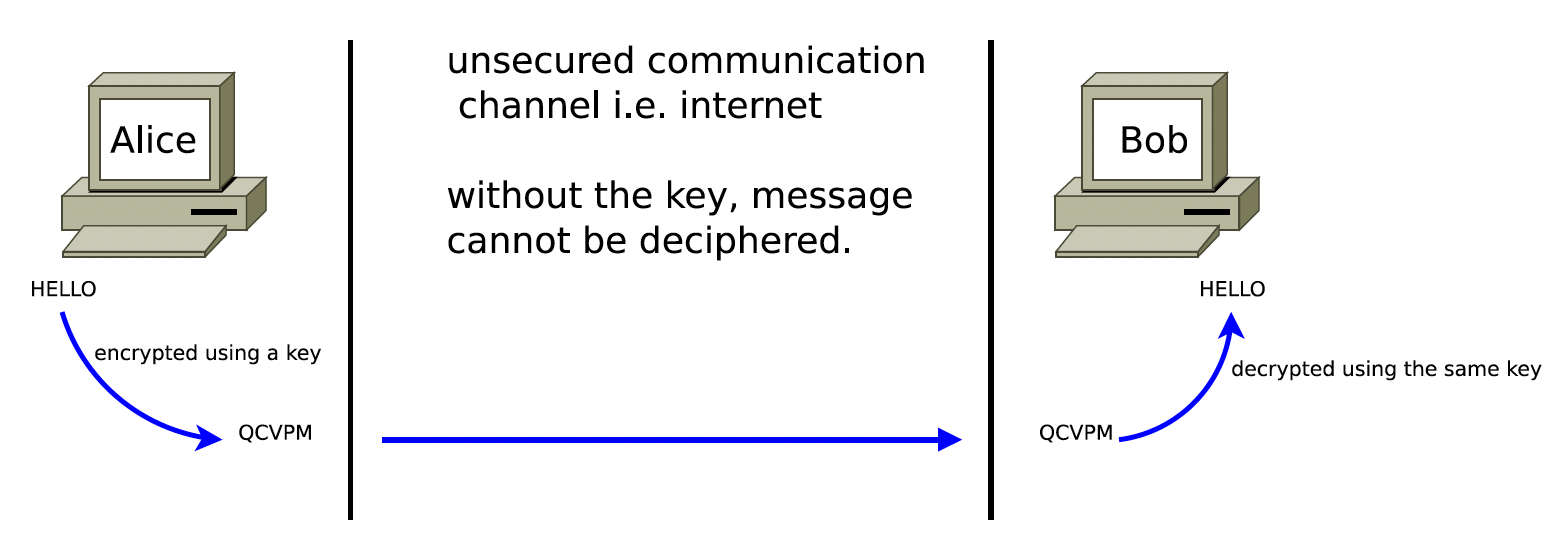
\includegraphics[keepaspectratio]{2.png}}\\
Asymmetric cryptography is relatively newer and uses the idea of two
keys. The two keys are linked in such a way that any message encrypted
with one of them requires the second to be decrypted. Another
characteristic of the keys is that you can not design (or guess) one of
them from the other. This second characteristic is the whole crux of the
system. One of the more common ways of guaranteeing that is the use of
prime numbers/factors. It takes very long to identify whether a number
is prime, and it takes even longer to identify the prime factors of a
number (particularly a very large number). The process of
encryption/decryption is therefore slightly different. The person who
wants to send a message encrypts it with one key, and the person who
wants to decrypt it uses the other key. The first key is called the
public key because you provide that key to everyone and anyone. You do
this so that anyone who wants to send you a message can be sure that you
are the only person who can open it since you are the only person who
has the other key (aptly called the private key)
\pandocbounded{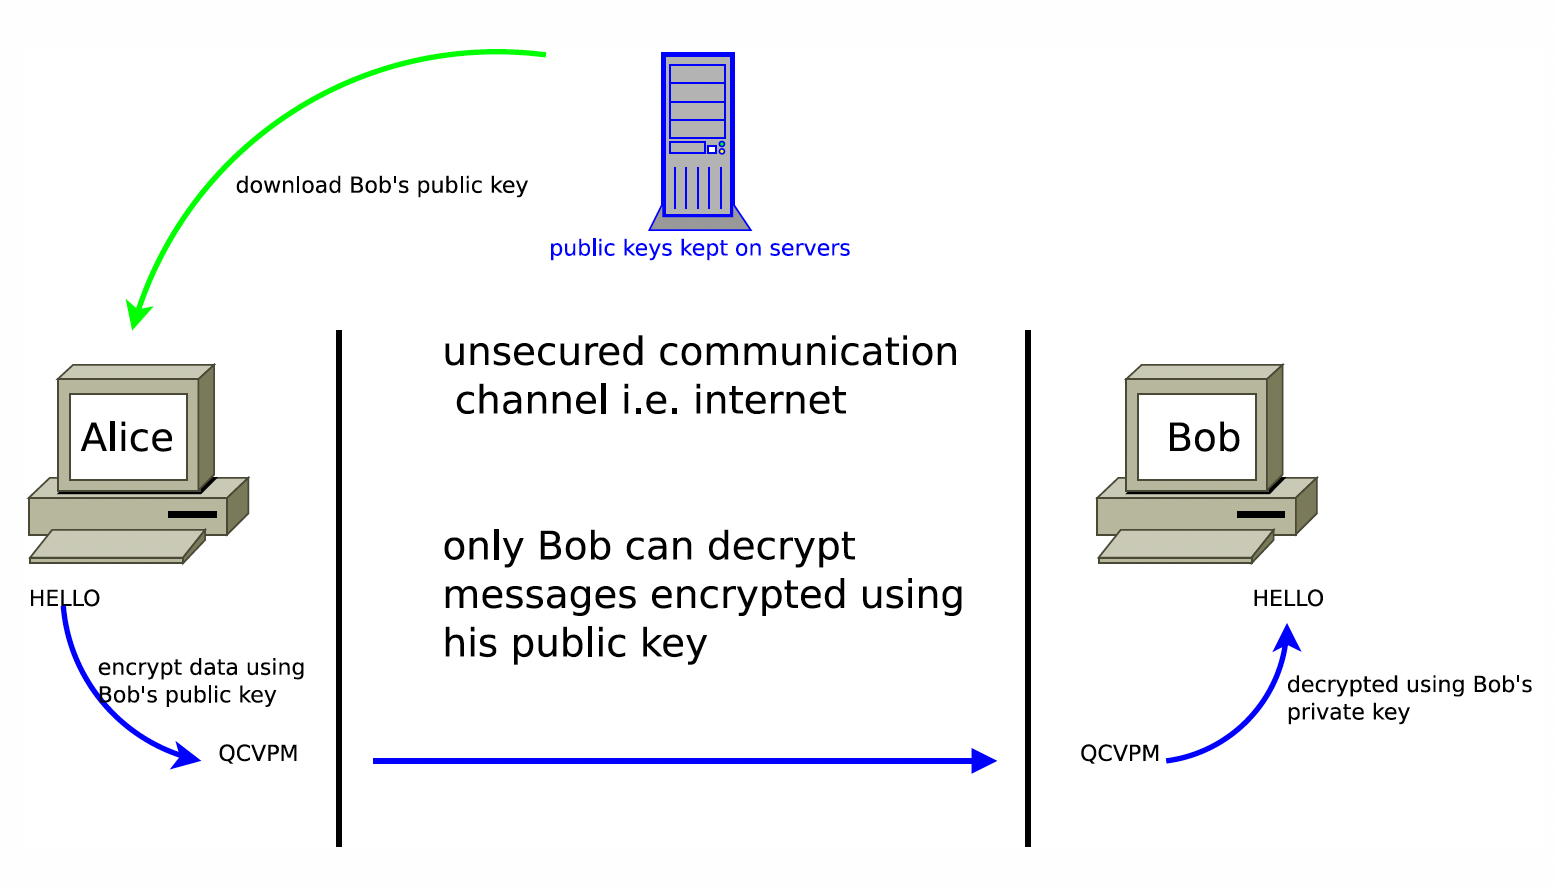
\includegraphics[keepaspectratio]{3.png}}

There are two major advantages of this approach. First is that we don't
have to have met for you to communicate with me and know that our
communication is private. There are servers dedicated to storing
people's public keys, people attach them to emails, etc. So if you want
to communicate with me, all I have to have done is have published my
public key somewhere.\\
\strut \\
The second advantage is that this technique allows us to solve the
problem of confirming the identity of someone if the
encryption/decryption process is reversed. Person A uses their private
key to encrypt a broadcast message. Anyone who has access to their
public key (which everyone does) can now use that key to decrypt the
message. It might be weird because it is not a secret message and anyone
can decrypt it but the cool thing about it is that we all know that
no-one else could have created that message in the first place since
only you have the private key. In that regard, the public/private key
approach allows us to have digital signatures which help us to determine
the authenticity of a message. It allows us to answer questions like
``is this message from a trusted source?'' and ``has this message been
changed in transit by someone pretending to be the trusted source?''.\\
\strut \\
Examples of the public/private key systems include Diffie-Helman, RSA,
DSA (Digital Signature algorithm), ECDSA (Eliptical curve DSA). You can
find some of these details in the certificate details of your web
browser.\\
\strut \\
Hashing is another way cryptography is used today. Recall from CSC 220
that hashing is a central part of how hash tables work. For hash tables,
hashing converted a key of any length/type into a valid index in the
table where the value would be stored. Outside of hash tables, hashing
is used to translate data of any size into a unique fixed size string
output. Any good hashing function works in such a way that this process
cannot be reversed. At first glance, this seems counter productive
i.e.~why scramble up a long message into a short string of gibberish if
I cannot unscramble that gibberish back to get the message? The reason
is that a good hash function will scramble any message into a unique
string of gibberish. I'll give you two examples of where this
functionality is actually helpful.\\
\strut \\
Imagine you downloaded an ISO file for Linux Mint and it took 2 hours to
download on your home internet (in fact imagine how long it would take
on the slow internet we had not that long ago). It would be very painful
if you took a full day installing the operating system only to realise
that the ISO file was corrupted in some way during the download and
you'll have to start the whole download and install process again with
the hope that it doesn't happen again. What many servers that store
large files will do is provide a hash of that file. That way once you
have downloaded the file, you can run it through the hash function, a
process which takes a very short time, and confirm if the hash you got
is identical to the hash that the server said you should get. If so,
then your file was not corrupted. If not, then you need to re-download
and not waste your time installing the corrupted file.\\
\strut \\
Another place that hashing is used is in the storage of passwords. Given
that bad actors can easily get access to systems, it would be bad if
they got access to every password that was ever used on that system in
plain text. What most servers/systems will do is actually store a hash
of your password instead. That way there is no way the bad actors can
get your passwords. They just get the hashes and there is no way to get
the passwords when you have the hash. The only thing they can do is run
a bunch of passwords they know of through the hashing function and hope
that one of them hashes to the exact same thing as your hash. And if
that happens then they have figured out your password. There are ways to
deal with this but they are beyond our discussion right now.\\
\strut \\
There are multiple hashing functions being used these days. These hash
functions are typically evaluated based on the number of collisions they
have (which should be very low), and how difficult they are to reverse
(which should be impossible).\\
\strut \\
MD5 (Message Digest algorithm 5) converts large data into a string of
128 bits. As early as 1993 researchers found vulnerabilities in it (such
as collisions) and so it isn't used much for high security cryptography
but rather for checksums to verify data.

\begin{Shaded}
\begin{Highlighting}[]
\NormalTok{$ echo {-}n "hello world" | md5sum \# any small difference in input}
\NormalTok{$ echo “hello world” | md5sum \# should produce a very different hash}
\end{Highlighting}
\end{Shaded}

SHA -- Secure Hash Algorithms -- is a family of hashing functions. SHA1
is similar to MD5 and was pretty much abandoned as of 2010. SHA 256 and
SHA 512 are probably some of the more common ones and are named after
the length in bits of the output they produce.

\begin{Shaded}
\begin{Highlighting}[]
\NormalTok{$ echo {-}n "hello world" | sha1sum}
\NormalTok{$ echo {-}n “hello world” | sha256sum}
\NormalTok{$ echo {-}n “hello world” | sha512sum}
\end{Highlighting}
\end{Shaded}

This has been a lot of information but hopefully it is very intriguing
information. Some of these topics we shall cover in more detail later in
the quarter with more application. Others you'll just have to wait till
you see them in classes like CSC 444/544/CYEN 406 \footnote{Typically
  offered every other year in the Spring quarter. Was last offered in
  Spring 2024.}.




\end{document}
